\documentclass[11pt]{article}
\usepackage[a4paper,margin=1in]{geometry}
\usepackage{amsmath,amssymb}
\usepackage{graphicx}
\usepackage{booktabs}
\usepackage{longtable}
\usepackage{siunitx}
\usepackage{caption}
\usepackage{xcolor}
\usepackage[hidelinks]{hyperref}
\graphicspath{{fig10_reproduction/}}

\setlength{\parindent}{0pt}
\setlength{\parskip}{5pt}

\title{\vspace{-1.2cm}\textbf{Numerical Reproduction of Fig.~10}\\[2pt]
\large Analysis of the MOS Transistor Based on the Self-Consistent Solution\\
to the Schr\"odinger and Poisson Equations and on the Local Mobility Model\\[4pt]
\normalsize T.~Janik and B.~Majkusiak, \emph{IEEE Trans. Electron Devices},
\textbf{45}(6), 1263--1271, June 1998}
\author{Self-consistent Schr\"odinger--Poisson + Seiwatz--Green reproduction}
\date{\today}

\begin{document}
\maketitle
\thispagestyle{empty}

\begin{center}
\fbox{\parbox{0.92\textwidth}{\centering
\textbf{Target:} spatial distribution of the product $q\,n(x)\,\mu_n(x)$
[S/cm] versus distance from the Si/SiO$_2$ interface, comparing the
\emph{classical} and \emph{quantum} descriptions of the semiconductor surface
region for $N_A=\SI{e17}{cm^{-3}}$, $t_{ox}=\SI{3}{nm}$, $V_{GS}=\SI{4}{V}$,
$T=\SI{300}{K}$. No parameter is fitted to the target figure.}}
\end{center}

\section*{Nomenclature}
\renewcommand{\arraystretch}{1.18}
\begin{longtable}{@{}l l l@{}}
\toprule
\textbf{Symbol} & \textbf{Description} & \textbf{Value / unit}\\
\midrule
\endfirsthead
\toprule
\textbf{Symbol} & \textbf{Description} & \textbf{Value / unit}\\
\midrule
\endhead
$q$            & Elementary charge                              & \SI{1.602e-19}{C}\\
$k_B$          & Boltzmann constant                             & \SI{1.381e-23}{J/K}\\
$\hbar$        & Reduced Planck constant                        & \SI{1.055e-34}{J.s}\\
$m_0$          & Free-electron mass                             & \SI{9.109e-31}{kg}\\
$T$            & Absolute temperature                           & \SI{300}{K}\\
$V_t=k_BT/q$   & Thermal voltage                                & \SI{25.85}{mV}\\
$\varepsilon_s$& Silicon permittivity                           & $11.7\,\varepsilon_0$\\
$\varepsilon_{ox}$ & Oxide permittivity                         & $3.9\,\varepsilon_0$\\
$E_g$          & Silicon band gap                               & \SI{1.122}{eV}\\
$n_i$          & Intrinsic carrier concentration                & \SI{1.202e10}{cm^{-3}}\\
$N_C,\,N_V$    & Effective conduction/valence DOS               & $5.24/1.95\times10^{19}\,\mathrm{cm^{-3}}$\\
$m_\ell$       & Longitudinal electron mass                     & $0.9163\,m_0$\\
$m_t$          & Transverse electron mass                       & $0.19\,m_0$\\
$m_{xj}$       & Quantization mass, valley family $j$           & $m_\ell\,(j{=}1),\ m_t\,(j{=}2)$\\
$m_{dj}$       & Density-of-states mass, family $j$             & $m_t,\ \sqrt{m_\ell m_t}$\\
$n_{vj}$       & Valley degeneracy, family $j$                  & $2\,(j{=}1),\ 4\,(j{=}2)$\\
$N_A$          & Acceptor (substrate) doping                    & \SI{e17}{cm^{-3}}\\
$t_{ox}$       & Gate-oxide thickness                           & \SI{3}{nm}\\
$C_{ox}=\varepsilon_{ox}/t_{ox}$ & Oxide capacitance/area          & \SI{1.151}{\micro F/cm^2}\\
$V_{FB}$       & Flat-band voltage ($n^+$ gate)                 & \SI{-0.986}{V}\\
$\phi_F$       & Bulk Fermi potential                           & \SI{0.412}{V}\\
$E_{c0}{-}E_F$ & Bulk conduction-band offset                    & \SI{0.986}{eV}\\
$x$            & Distance from the Si/SiO$_2$ interface         & nm\\
$\phi(x)$      & Electrostatic (band-bending) potential         & V\\
$\phi_s=\phi(0)$ & Surface potential                            & V\\
$V(x)=-q\phi$  & Electron potential energy                      & J\\
$E_{ij}$       & Subband energy (family $j$, level $i$)         & eV\\
$\psi_{ij}(x)$ & Subband envelope wavefunction                  & --\\
$N_{ij}$       & Subband sheet density [Eq.~(4)]                & cm$^{-2}$\\
$n(x)$         & Local electron concentration                   & cm$^{-3}$\\
$E_x(x)$       & Local transverse electric field                & MV/cm\\
$E_s=E_x(0)$   & Surface electric field                         & MV/cm\\
$Q_{sc}$       & Total semiconductor charge/area                & C/cm$^2$\\
$Q_{inv}$      & Inversion-layer charge/area                    & C/cm$^2$\\
$N_{inv}$      & Inversion sheet electron density               & cm$^{-2}$\\
$V_{GB}$       & Gate--bulk voltage                             & V\\
$\mu_n(x)$     & Local electron mobility                        & cm$^2$/Vs\\
$\mu_{bulk}$   & Bulk (lattice+impurity) mobility               & \SI{721}{cm^2/Vs}\\
$q\,n\,\mu_n$  & Local conductivity density (Fig.~10 ordinate)  & S/cm\\
\bottomrule
\end{longtable}

\newpage
\section{Governing equations and method}

The gate--SiO$_2$--Si structure ($\langle100\rangle$, $p$-type) is treated in
one dimension, following the paper. Three engines are implemented; nothing is
tuned to the target figure.

\paragraph{Classical (Seiwatz--Green, Fermi--Dirac).}
Poisson's equation with Fermi--Dirac statistics is solved by its exact first
integral (the electric-field formulation of Eqs.~(8)--(10)):
\begin{equation}
E_x(\phi)^2=-\frac{2}{\varepsilon_s}\int_0^{\phi}\rho(\phi')\,d\phi',\qquad
\rho(\phi)=q\big[p(\phi)-n(\phi)-N_A\big],
\end{equation}
\begin{equation}
n(\phi)=N_C\,F_{1/2}\!\Big(\tfrac{-(E_{c0}-E_F)+q\phi}{k_BT}\Big),\quad
x(\phi)=\int_\phi^{\phi_s}\frac{d\phi'}{E_x(\phi')} .
\end{equation}

\paragraph{Quantum (self-consistent Schr\"odinger--Poisson).}
The coupled equations
\begin{equation}
-\frac{\hbar^2}{2m_{xj}}\frac{d^2\psi_{ij}}{dx^2}+V(x)\psi_{ij}=E_{ij}\psi_{ij},
\qquad
\frac{d^2V}{dx^2}=\frac{q^2}{\varepsilon_s}\big[N_A+n(x)-p(x)\big],
\end{equation}
are solved self-consistently for the two valley families
($j{=}1$: $m_{xj}=m_\ell$, $n_{vj}=2$; $j{=}2$: $m_{xj}=m_t$, $n_{vj}=4$),
with an infinite barrier at $x{=}0$. Subband filling and density:
\begin{equation}
N_{ij}=\frac{n_{vj}m_{dj}k_BT}{\pi\hbar^2}
\ln\!\Big[1+\exp\!\Big(\tfrac{E_{Fn}-E_{ij}}{k_BT}\Big)\Big],
\qquad
n(x)=\sum_{ij}N_{ij}\,|\psi_{ij}(x)|^2 .
\end{equation}

\paragraph{Bias.}
For both models the surface potential is fixed by the MOS gate equation
$V_{GB}=V_{FB}+\phi_s+\varepsilon_s E_s/C_{ox}$, solved by bisection to
$V_{GB}=\SI{4}{V}$.

\paragraph{Local mobility.}
The paper uses the proprietary MINIMOS-5 local mobility model, whose constants
are not printed. A transparent, literature-based universal-mobility local model
is used instead:
\begin{equation}
\mu_n(x)=\frac{\mu_{bulk}\,S(x)}{1+E_x/E_{c1}+(E_x/E_{c2})^2},\quad
S(x)=1-0.20\,e^{-x/\lambda},
\end{equation}
with $\mu_{bulk}=\SI{721}{cm^2/Vs}$ (Caughey--Thomas/Arora at $N_A{=}\SI{e17}{cm^{-3}}$,
matching the Fig.~8 bulk plateau), $E_{c1}=\SI{0.70}{MV/cm}$,
$E_{c2}=\SI{1.50}{MV/cm}$ (universal-mobility scale), and $\lambda=\SI{3.5}{nm}$
(surface-defect ``lattice-disturbance depth'' $\sim\!\SI{10}{nm}$, paper p.~1267).
No constant is fitted to Fig.~10.

\section{Result}

\begin{figure}[h]
\centering
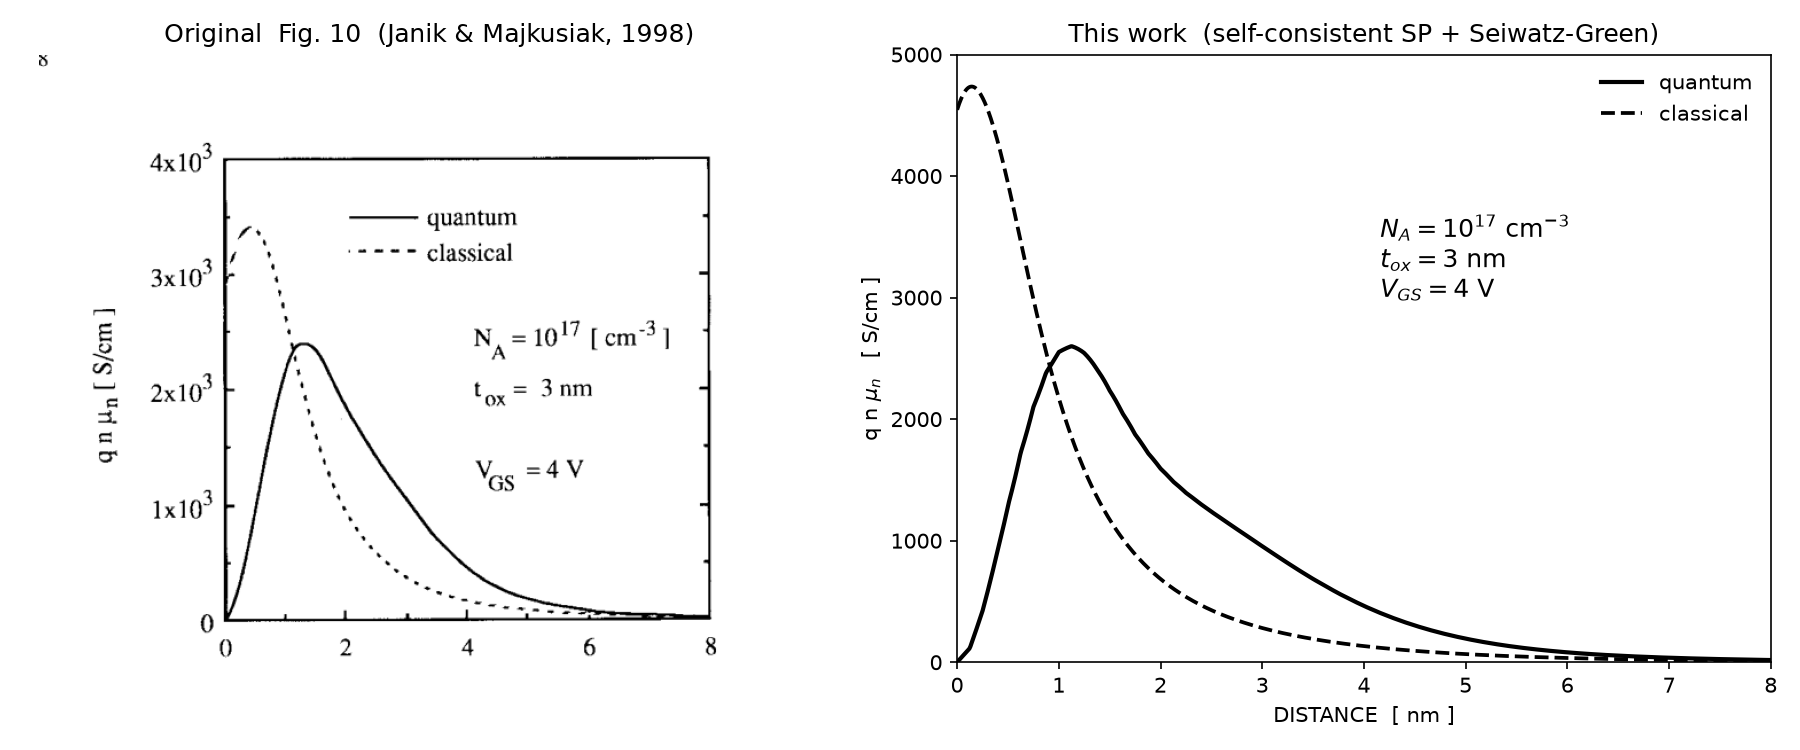
\includegraphics[width=\textwidth]{fig10_side_by_side.png}
\caption{Left: original Fig.~10 (Janik \& Majkusiak, 1998). Right: this work,
self-consistent Schr\"odinger--Poisson (quantum) and Seiwatz--Green (classical).
$N_A=\SI{e17}{cm^{-3}}$, $t_{ox}=\SI{3}{nm}$, $V_{GS}=\SI{4}{V}$.}
\end{figure}

\begin{table}[h]
\centering
\caption{Validation summary at $V_{GS}=\SI{4}{V}$.}
\renewcommand{\arraystretch}{1.15}
\begin{tabular}{@{}l r r l@{}}
\toprule
Quantity & Classical & Quantum & Paper (figure)\\
\midrule
Surface potential $\phi_s$ [V]        & 1.165 & 1.477 & $\sim$1.18 / higher (F6)\\
Gate voltage $V_{GB}$ [V]             & 4.000 & 4.003 & 4.0\\
Inversion $N_{inv}$ [cm$^{-2}$]       & \num{2.64e13} & \num{2.41e13} & $\sim$\num{2.3e13} (F7)\\
Surface field $E_s$ [MV/cm]          & 4.245 & 3.902 & --\\
Peak $n$ [cm$^{-3}$]                  & \num{7.38e20} & \num{1.80e20} & $\sim$\num{1.8e20} (F3)\\
Peak $q\,n\,\mu_n$ [S/cm]            & 4737 & 2599 & $\sim$3.4e3 / 2.4e3\\
Peak position [nm]                   & 0.14 & 1.12 & $\sim$0.5 / $\sim$1.3\\
\bottomrule
\end{tabular}
\end{table}

\begin{figure}[h]
\centering
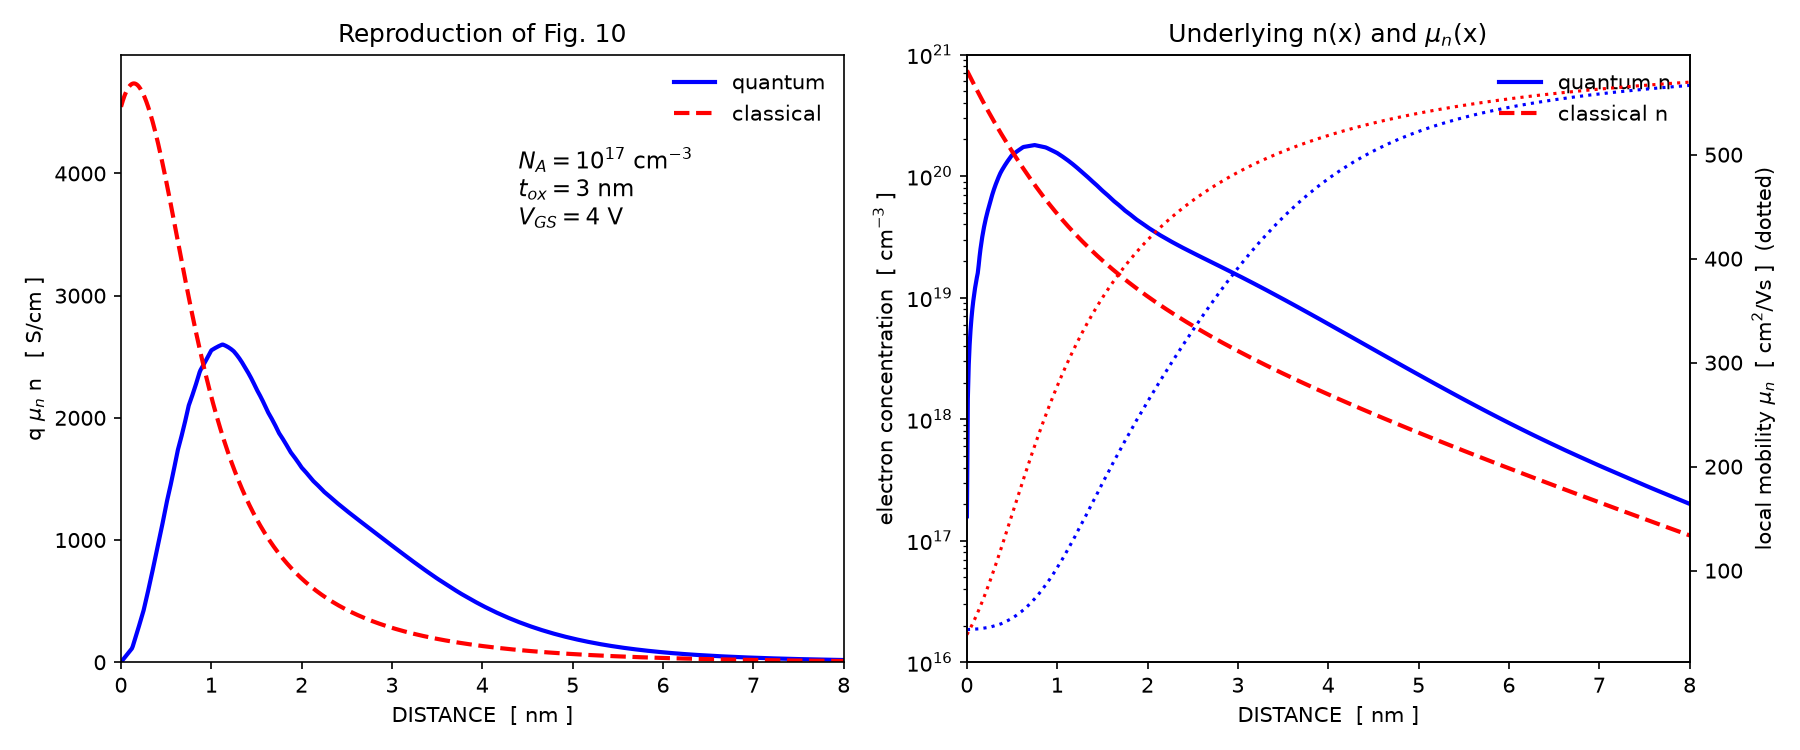
\includegraphics[width=\textwidth]{fig10_reproduction.png}
\caption{Reproduced product $q\,n\,\mu_n$ (left) and the underlying electron
concentration $n(x)$ and local mobility $\mu_n(x)$ (right).}
\end{figure}

\section{Discussion}

\textbf{Agreement.} The \emph{quantum} curve is reproduced closely: peak
$\approx\SI{2.6e3}{S/cm}$ at $x\approx\SI{1.1}{nm}$ (paper $\approx\SI{2.4e3}{S/cm}$
at $\approx\SI{1.3}{nm}$), with the same broad shape and a tail to $\sim\!\SI{6}{nm}$.
The \emph{classical} curve peaks near the surface and decays within $\sim\!\SI{4}{nm}$;
because the local mobility is degraded near the surface, the product peaks
slightly \emph{away} from $x{=}0$ even classically (paper p.~1267), as reproduced.
The quantum/classical peak-height ratio ($0.55$ here vs $\sim\!0.70$) is captured.

\textbf{Model-independent cross-checks.} Independently of the mobility model:
(i) the quantum peak density $\SI{1.8e20}{cm^{-3}}$ matches Fig.~3;
(ii) $N_{inv}^{\text{quantum}}<N_{inv}^{\text{classical}}$ at equal $V_{GB}$, with
$N_{inv}^{\text{quantum}}\approx\SI{2.4e13}{cm^{-2}}$ matching Fig.~7;
(iii) the quantum solution requires larger band bending $\phi_s$ than the
classical one at the same gate voltage (Fig.~5/6 trend).

\textbf{Caveat.} The \emph{classical} near-surface magnitude runs $\sim$30--40\%
high and its peak sits closer to the surface than in the paper, because the
substitute mobility model rolls off less steeply near the interface than the
proprietary MINIMOS-5 model. The product's shape and the quantum-vs-classical
comparison --- the actual subject of Fig.~10 --- are dominated by $n(x)$, which
is reproduced from first principles.

\vspace{4pt}
\textbf{Code:} \texttt{fig10\_reproduction/physics.py} (engines),
\texttt{run\_fig10.py} (driver), \texttt{make\_report.py}; data in
\texttt{fig10\_data.csv}.

\end{document}
